\documentclass[10pt]{article}

\PassOptionsToPackage{numbers,compress}{natbib}
\usepackage[utf8]{inputenc}
\usepackage[T1]{fontenc}
\usepackage{hyperref}
\usepackage{url}
\usepackage{booktabs}
\usepackage{amsfonts}
\usepackage{amsmath}
\usepackage{amssymb}
\usepackage{microtype}
\usepackage{xcolor}
\usepackage{graphicx}
\usepackage{subcaption}
\captionsetup{font=small,skip=3pt}
\usepackage{natbib}
\usepackage{times}
\usepackage{enumitem}
% NeurIPS-style geometry: 5.5" text width, 9" text height, 1.5" left margin
\usepackage[
  letterpaper,
  left=1.5in, right=1.5in,
  top=1.0in,  bottom=1.0in,
  headheight=12pt
]{geometry}

\hypersetup{colorlinks=true,linkcolor=blue,citecolor=blue,urlcolor=blue}
% NeurIPS paragraph style: no indent, compact spacing
\setlength{\parindent}{0pt}
\setlength{\parskip}{4pt}
\setlist[itemize]{leftmargin=1.2em,itemsep=0.05em,topsep=0.2em}
\setlist[enumerate]{leftmargin=1.3em,itemsep=0.05em,topsep=0.2em}
% Allow more floats per page so fig2+fig3 co-locate on page 6
\renewcommand{\topfraction}{0.92}
\renewcommand{\textfraction}{0.08}
\setlength{\floatsep}{6pt plus 2pt minus 2pt}
\setlength{\textfloatsep}{8pt plus 2pt minus 2pt}

% NeurIPS-style title formatting
\usepackage{titlesec}
% First-level: bold, 12pt, lower case (first word + proper nouns only)
\titleformat{\section}{\normalfont\large\bfseries}{\thesection}{1em}{}
\titlespacing*{\section}{0pt}{8pt plus 2pt minus 1pt}{4pt plus 1pt minus 1pt}
% Second-level: bold, 10pt
\titleformat{\subsection}{\normalfont\normalsize\bfseries}{\thesubsection}{1em}{}
\titlespacing*{\subsection}{0pt}{6pt plus 1pt}{2pt plus 1pt}

\title{\textbf{When does graph propagation help causal recommendation?}\\[0.3em]
\large A randomized-test mechanism study on exposure-biased user--item graphs}
\author{Kien Lau \\
  Yale University \\
  \texttt{kien.lau@yale.edu}
}
\date{April 24, 2026}

\begin{document}
\maketitle

\begin{abstract}
Recommendation logs are missing-not-at-random: users rate items they were exposed to, not a random sample of what they might like. Graph collaborative filtering then propagates over this biased graph, which may help by sharing preference signal or hurt by amplifying exposure bias. The analysis isolates the mechanism using two randomized-test benchmarks: Coat and the full Yahoo! R3 dataset. Across a matched zero-hop baseline, LightGCN depths $K\in\{1,2,3\}$, and two popularity-tempered residual variants, graph propagation improves randomized-test ranking on both datasets. The larger Yahoo dataset on 311{,}704 observational ratings and 54{,}000 randomized-test ratings shows $K=1$ improves NDCG@5 from 0.653 to 0.679, while deeper propagation increases popularity shift and eventually loses accuracy. A simple degree penalty does not solve the problem: it reduces some shift relative to vanilla $K=2$ but lowers NDCG on both datasets. The conclusion is therefore conditional but clear: propagation helps causal recommendation, but popularity correction requires more than a local degree transformation.
\end{abstract}

\section{Introduction}
\label{sec:intro}

Recommendation systems are causal systems: a click or rating is observed only after a platform exposes user $u$ to item $i$. Standard logs mix preference with the platform's prior policy and item popularity. A model that performs well on those same logs may simply reproduce exposure patterns, leading to over-recommending head items while appearing accurate offline.

The user--item graph is not a neutral sample of unobserved, latent preferences. An observed edge means that an item was both exposed and rated; a missing edge does not mean dislike, only that the rating was not observed. This is the missing-not-at-random (MNAR) setting: the observation process depends on the platform policy, item visibility, and user behavior rather than on independent random sampling. As a result, graph topology contains two entangled signals: who might like what, and who was given the opportunity to express that preference.

This matters directly for graph collaborative filtering (GCF). Methods such as LightGCN~\citep{he2020} improve recommendation by propagating embeddings over the observed bipartite graph, letting users borrow signal from neighboring items and other users. This propagation, however, treats the observed graph as unbiased for message passing. If popular items are over-represented because they were shown more often, multi-hop aggregation can route this exposure bias through the graph and make recommendations look better on historical observed splits without improving what would happen under a less biased exposure process. The core problem is not simply link prediction on a sparse bipartite graph. The target is a user--item ranking model whose test set answers the question: if this user were shown this item, would the user rate it favorably?

Randomized-test recommendation benchmarks create a useful stress test for this mechanism. They do not make the observational training graph unbiased, and they do not by themselves identify every causal effect. 

These benchmarks allow for evaluation of rankings on items assigned outside of the usual platform-exposure process. Fundamentally, the study shifts the question from ``can a graph model reconstruct logged edges?'' to ``does graph propagation still help when the evaluation is on randomized exposure?'' That distinction is important because propagation has two plausible effects. One plausible effect is that it improves ranking by sharing genuine collaborative signal across similar users and items. The other effect is that it amplifies exposure bias by repeatedly averaging over a graph whose high-degree nodes are high-degree partly because they were visible in the first place.

The study considers two questions with matched controls on randomized-test data:

\begin{enumerate}
  \item \textbf{RQ1:} Does multi-hop graph propagation improve randomized-test ranking over a matched zero-hop embedding model?
  \item \textbf{RQ2:} Can a lightweight popularity-tempered propagation correction simultaneously improve randomized-test NDCG and reduce popularity amplification relative to vanilla propagation?
\end{enumerate}

The model is tasked with ranking candidate items for each user from user and item embeddings. The experimental design holds the loss, optimizer, embedding size, and training positives fixed, varying only the propagation depth: zero-hop matrix-factorization-style embeddings, LightGCN with depths $K\in\{1,2,3\}$, and two degree-tempered residual propagation variants. Coat provides a small but seed-averaged benchmark; Yahoo! R3 provides a larger external-validity check. The results show that propagation improves randomized-test ranking on both datasets, but Yahoo shows that deeper propagation increases popularity shift and eventually loses accuracy. Additionally, simply penalizing node degree does not preserve the ranking gains from vanilla propagation.

\section{Related work}
\label{sec:related}

The MNAR recommendation literature explains why ordinary offline splits can be misleading. Marlin and Zemel~\citep{marlin2009} studied collaborative prediction and ranking when ratings are not missing at random, showing that learning from observed ratings alone can pass missingness bias into predictions and rankings. Steck~\citep{steck2010} similarly treated absent ratings as informative rather than ignorable and proposed evaluation/training ideas for MNAR recommendation. These papers establish the statistical problem, but they do not focus on modern graph propagation architectures.

Schnabel et al.~\citep{schnabel2016} made the causal framing explicit by treating recommendation exposure as a treatment and adapting inverse-propensity ideas for debiased learning and evaluation. Wang et al.~\citep{wang2020} sharpened this view by asking the counterfactual question of how a user would rate an item under forced exposure, and they used Coat and Yahoo! R3 random test sets to evaluate deconfounded recommendation models. More recent work studies harder forms of the same problem, including hidden confounding~\citep{zhang2023,li2023} and interference or neighborhood effects~\citep{li2024}. The present study builds on their causal-evaluation work, but it is narrower. Rather than identifying causal effects from observational graphs, the randomized-test data are used as a target for mechanistic study of graph propagation.

Graph recommenders address a different gap: how to exploit high-order structure in user--item interactions. PinSage showed that graph convolutions and random-walk neighborhoods can scale to web-scale recommendation~\citep{ying2018}. NGCF explicitly encoded high-order collaborative signal through embedding propagation on the user--item graph~\citep{wang2019}. LightGCN then simplified this idea by removing feature transformations and nonlinearities that contributed little for collaborative filtering, leaving a clean propagation-and-layer-averaging model~\citep{he2020}. SimGCL is another example of the field's emphasis on representation learning over the interaction graph, using a simple contrastive approach to improve accuracy and efficiency~\citep{yu2022}. These models motivate the simple, baseline architecture here: if propagation is the core operation, then its effect should be isolated from unrelated choices such as embedding size, loss, or optimizer.

Recent graph-side debiasing work is closest to the present study. Kim et al.~\citep{kim2022} argue that exposure bias can enter not only through the final loss but also through neighbor aggregation itself, and propose propensity-weighted aggregation. Zhang et al.~\citep{zhang2024} similarly target bias in graph-based collaborative filtering by separating bias-aware and bias-mitigated graph views through adversarial graph dropout. Compared with these methods, this study deliberately tests a simpler question: before adding a full debiasing pipeline, does vanilla propagation actually help under randomized evaluation, and can a minimal degree-based correction reduce popularity amplification without sacrificing NDCG?

\section{Causal setup and data}
\label{sec:setup}

\textbf{Causal framing.} The fundamental question for recommendation evaluation is: if user $u$ were shown item $i$ at random, would they rate it favorably? Let $Y_{ui}(1)$ denote this potential outcome under forced exposure. The interaction logs only reveal ratings for items users were actually exposed to, so the observed rating can be written as $R_{ui} = O_{ui} \cdot Y_{ui}(1)$ where $O_{ui}\in\{0,1\}$ is the exposure indicator. The training graph $G_{\text{obs}}=(\mathcal U\cup\mathcal I,\,E_{\text{obs}})$ collects all observed interactions: $E_{\text{obs}}=\{(u,i):O_{ui}=1\}$.

Since exposure depends on the platform's recommendation policy and users' prior behavior, the training graph is generated by the logging distribution $p_{\text{log}}(u,i)\propto\Pr(O_{ui}=1)$. The target quantity, however, is the ranking risk under a randomized distribution $p_{\text{rand}}(u,i)$:
\[
  \mathcal{R}(f) = \mathbb{E}_{(u,i)\sim p_{\text{rand}}}\bigl[\ell\{Y_{ui}(1),\,f(u,i)\}\bigr].
\]
A randomized test set approximates samples from $p_{\text{rand}}$ and supports empirical evaluation of $\mathcal{R}(f)$. This study does not claim full causal identification from the observational training graph; the randomized test split is used purely as an intervention-like evaluation target.

\textbf{Datasets and splits.} Coat~\citep{schnabel2016} is a product-rating dataset with 290 users and 300 coat items. Its observational split contains user-selected ratings, while its randomized split contains 16 randomly assigned test ratings per user. Yahoo! R3~\citep{yahoor3kaggle} is a music-rating dataset; it contains \texttt{user.txt} with 311{,}704 user-supplied ratings and \texttt{random.txt} with 54{,}000 randomized ratings from 5{,}400 users over 1{,}000 songs. 


For both datasets, the observational/MNAR split is used for training and the randomized split is used only for final evaluation. No separate validation split was used for hyperparameter tuning because the study compares a fixed set of propagation operations rather than a large hyperparameter search space. Since the datasets are interaction graphs, the useful raw information is on user-item edges: the rating value. All ratings are converted to the same binary label, $y_{ui}=1$ iff $rating_{ui}\ge3$. The Yahoo dataset did not have user/item features. We intentionally use only learned ID embeddings to isolate the effect of graph propagation over the interaction topology. Adding features in the Coat dataset, would introduce another source of signal and make it harder to tell whether performance changes come from propagation or from features.



\begin{table}[t]
\centering
\small
\caption{Dataset statistics. Density uses active users for each split. Standard triangle clustering is not meaningful for strict bipartite user--item graphs, so head-item concentration summarizes the degree distribution.}
\label{tab:data}
\begin{tabular}{llrrrrrr}
\toprule
Data & Split & Users & Items & Edges & Density & Pos.\ rate & Top 10\% \\
\midrule
Coat & MNAR train & 290 & 300 & 6{,}960 & 0.080 & 0.520 & 0.236 \\
Coat & Random test & 290 & 300 & 4{,}640 & 0.053 & 0.401 & 0.146 \\
Yahoo & MNAR train & 15{,}400 & 1{,}000 & 311{,}704 & 0.020 & 0.559 & 0.480 \\
Yahoo & Random test & 5{,}400 & 1{,}000 & 54{,}000 & 0.010 & 0.232 & 0.125 \\
\bottomrule
\end{tabular}
\end{table}

Table~\ref{tab:data} provides the EDA summary used for the graph task: node counts, edge counts, density, label balance, and a degree-distribution diagnostic. The graphs are sparse bipartite rating graphs, with density ranging from 0.010 to 0.080 across splits. Label balance also shifts across splits: Yahoo has a 55.9\% positive rate in observational training but only 23.2\% in randomized testing, while Coat decreases from 52.0\% to 40.1\%. On Yahoo, the top 10\% of items account for 48.0\% of training ratings but only 12.5\% of randomized-test ratings. This head-item concentration, visualized in Figure~\ref{fig:yahoo-shift}, is the most relevant degree-distribution evidence for the study because LightGCN propagates over exactly this biased topology.

\begin{figure}[t]
\centering
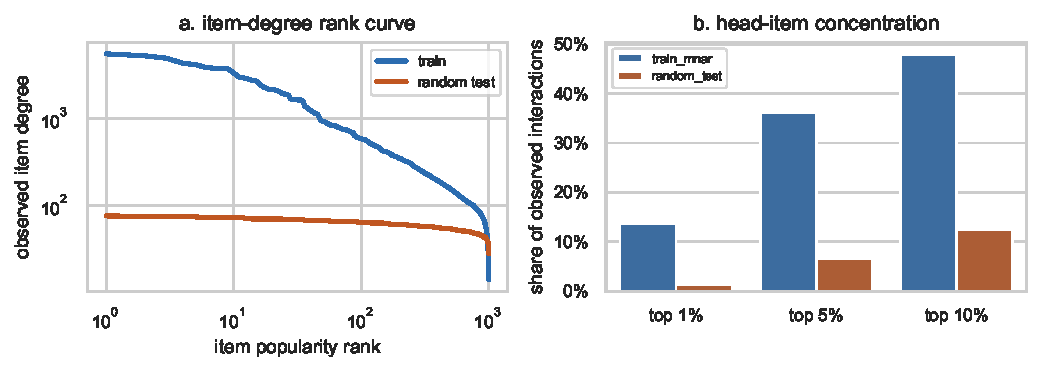
\includegraphics[width=\linewidth]{reproduceable_workspace/figures/yahoo_full/fig1_yahoo_smoke_popularity_shift.pdf}
\caption{Yahoo full-data exposure shift. The MNAR training split is far more head-concentrated than the randomized test split: the top 10\% of songs receive 48.0\% of train ratings but only 12.5\% of randomized-test ratings.}
\label{fig:yahoo-shift}
\end{figure}

\section{Method}
\label{sec:method}

All models share user and item embeddings $p_u,q_i\in\mathbb{R}^d$ with $d=32$ and scoring function $s_{ui}=p_u^\top q_i$. Training uses Bayesian personalized ranking (BPR):
\[
  \mathcal{L} = -\sum_{(u,i,j)}\log\sigma(s_{ui}-s_{uj}),
\]
where $i$ is a training-positive item ($r_{ui}\ge3$) and $j$ is a uniformly sampled non-positive item. Only the propagation operator differs across models; all other components are held fixed.

\textbf{Zero-hop control ($K=0$).} The baseline is a plain dot-product embedding model with no graph propagation and no neighborhood aggregation---identical to LightGCN at $K=0$. It establishes the performance attainable from memorized user and item embeddings alone, providing the controlled comparison for RQ1.

\textbf{Vanilla LightGCN ($K\in\{1,2,3\}$).} Embeddings are propagated over the normalized MNAR adjacency $\tilde{A}$:
\[
  H^{(k+1)} = \tilde{A}\,H^{(k)}, \qquad
  H_{\text{final}} = \frac{1}{K+1}\sum_{k=0}^{K}H^{(k)},
\]
where $\tilde{A}_{ui} = (d_u d_i)^{-1/2}$ for $(u,i)\in E_{\text{obs}}$. The depth sweep $K\in\{0,1,2,3\}$ is the primary ablation for RQ1; all hyperparameters other than $K$ are identical across depths.

\textbf{Popularity-tempered residual propagation.} To test RQ2, only the propagation weight is modified. A per-item degree penalty is introduced:
\[
  w_{ui}^{(\gamma)} = \frac{1}{\sqrt{d_u d_i}} \cdot \frac{1}{(d_i+1)^\gamma}, \qquad
  H^{(k+1)} = \lambda\,H^{(0)} + (1-\lambda)\,\tilde{A}_\gamma\,H^{(k)}.
\]
The factor $(d_i+1)^{-\gamma}$ down-weights messages from high-degree neighbors, and the residual coefficient $\lambda$ blends the original (unpropagated) embedding back in to limit overcorrection. To answer RQ2, two variants are tested at $K=2$: \textbf{Corrected A} ($\gamma=0.35, \lambda=0.20$) and \textbf{Corrected B} ($\gamma=0.70, \lambda=0.20$). This is a deliberately minimal intervention to test whether even a simple degree penalty at the propagation step suffices, before investing in full propensity-estimation pipelines.

\section{Experiments and results}
\label{sec:experiments}

\textbf{Experimental setup and baselines.} The comparison is an ablation over propagation rather than a broad model leaderboard. The zero-hop model is the baseline: it uses the same embeddings, BPR loss, optimizer, and training positives as LightGCN but performs no message passing. The main ablation compares vanilla LightGCN depths $K=1,2,3$ against that baseline. The two corrected models are the proposed lightweight intervention for RQ2, both at $K=2$.

All hyperparameters are fixed unless they define the ablation. The embedding dimension is 32, the optimizer is Adam with learning rate $3\times10^{-2}$ and weight decay $10^{-5}$, and training uses BPR. Coat uses batch size 1024, 180 epochs, and 20 seeds; Yahoo uses batch size 2048, 20 epochs, and one full-data seed. These settings were not selected by a large validation search; the goal is a controlled mechanism study where only propagation changes. All runs used CUDA on an NVIDIA GeForce RTX 3060. Runtimes are about 7--12 seconds per Coat run and 44--69 seconds per Yahoo full-data run.

\textbf{Metrics.} Models rank each user's randomized-test rated items. NDCG@5 rewards placing relevant items near the top; Recall@5 measures how many relevant randomized-test items appear anywhere in the top five. Popularity amplification is measured by top-5 head-item share and Jensen--Shannon (JS) divergence from the randomized-test item distribution. Lower head share and JS indicate less shift toward observational popularity, but they are interpreted with NDCG/Recall because reducing popularity is not useful if ranking quality collapses.

\begin{table}[t]
\centering
\small
\caption{Randomized-test results. Coat is mean over 20 seeds; Yahoo is one full-data run, no bootstraps. Head is top-5 head-item share.}
\label{tab:main}
\begin{tabular}{llcccc}
\toprule
Data & Model & NDCG@5 & Recall@5 & Head & JS \\
\midrule
Coat & 0-hop & $0.656\pm0.008$ & $0.474\pm0.011$ & 13.9\% & 0.042 \\
Coat & K1 & $0.672\pm0.006$ & $0.490\pm0.007$ & 14.6\% & 0.045 \\
Coat & K2 & $0.683\pm0.006$ & $0.503\pm0.007$ & 15.4\% & 0.054 \\
Coat & K3 & $\mathbf{0.689\pm0.005}$ & $\mathbf{0.510\pm0.006}$ & 15.9\% & 0.060 \\
Coat & Corr. & $0.675\pm0.007$ & $0.492\pm0.007$ & 14.7\% & 0.046 \\
Coat & Corr.+ & $0.673\pm0.007$ & $0.489\pm0.008$ & 14.6\% & 0.044 \\
\midrule
Yahoo & 0-hop & 0.653 & 0.700 & 16.8\% & 0.035 \\
Yahoo & K1 & \textbf{0.679} & 0.726 & 17.4\% & 0.046 \\
Yahoo & K2 & 0.673 & \textbf{0.729} & 18.2\% & 0.061 \\
Yahoo & K3 & 0.660 & 0.717 & 18.9\% & 0.074 \\
Yahoo & Corr. & 0.654 & 0.707 & 17.8\% & 0.056 \\
Yahoo & Corr.+ & 0.647 & 0.701 & 18.0\% & 0.061 \\
\bottomrule
\end{tabular}
\end{table}

\textbf{RQ1: depth ablation.} Propagation helps on both datasets, but the optimal depth differs. On Coat, NDCG rises from 0.656 at zero-hop to 0.689 at $K=3$ over 20 seeds. On Yahoo, $K=1$ improves NDCG from 0.653 to 0.679 over 3{,}922 evaluated users, while $K=2$ gives the best Recall@5. The Yahoo depth sweep also shows the failure mode: moving from $K=1$ to $K=3$ raises head share (17.4\% to 18.9\%) and JS (0.046 to 0.074), while NDCG falls from 0.679 to 0.660. Thus deeper propagation increasingly routes recommendations toward the MNAR training distribution while decreasing ranking quality.

\textbf{RQ2: correction ablation.} The degree correction changes the recommendation distribution but fails the accuracy criterion on both datasets. On Coat, the corrected variants reduce head share and JS relative to vanilla $K=2$, but NDCG drops below $K=2$ and also below $K=1$. On Yahoo, Corrected A reduces JS relative to vanilla $K=2$ (0.056 vs.\ 0.061), but NDCG falls from 0.673 to 0.654. Corrected B is worse. A local degree penalty can suppress some popularity shift, but it does not preserve the ranking benefit created by propagation.

\begin{figure}[!t]
\centering
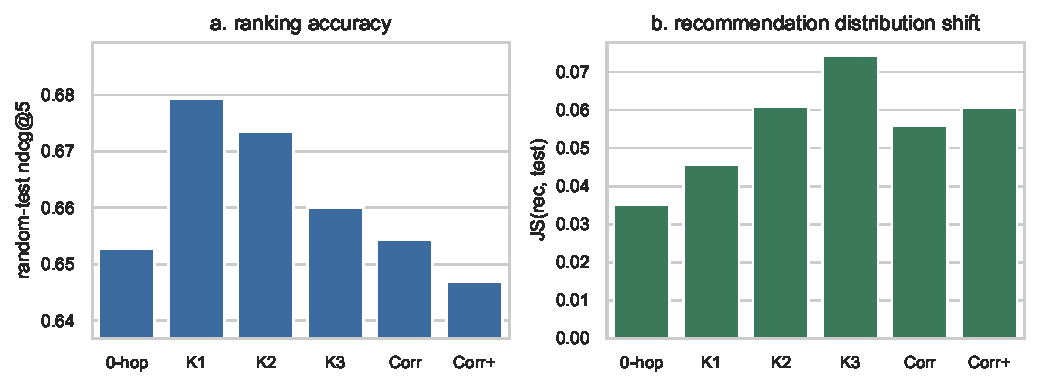
\includegraphics[width=\linewidth]{reproduceable_workspace/figures/yahoo_full/fig3_yahoo_smoke_accuracy_bias.pdf}
\caption{Yahoo full-data result. $K=1$ gives the best NDCG; $K=2$ gives the best Recall@5 (Table~\ref{tab:main}); deeper propagation increases recommendation-distribution shift. Corrected variants reduce some shift relative to vanilla $K=2$ but lose ranking accuracy.}
\label{fig:yahoo-results}
\end{figure}

\begin{table}[!h]
\centering
\small
\caption{Mechanism diagnostics from cached intermediate results. Yahoo degree values use the full-data run; Coat diagnostics use the 20-seed sample.}
\label{tab:mechanism}
\begin{tabular}{@{}p{0.20\linewidth}p{0.56\linewidth}r@{}}
\toprule
Claim & Diagnostic & Value \\
\midrule
Yahoo depth shift & Avg. train degree in top-5, K1 $\to$ K3 & 265.7 $\to$ 284.4 \\
Coat popularity signal & Spearman(train degree, random positive rate) & 0.191 \\
Coat head/tail preference & Random positive rate, tail $\to$ head quartile & 0.364 $\to$ 0.443 \\
Correction behavior & Avg. degree, vanilla-only $\to$ correction-only swaps & 12.53 $\to$ 10.04 \\
Correction error mode & Positive rate, vanilla-only $\to$ correction-only swaps & 0.447 $\to$ 0.401 \\
\bottomrule
\end{tabular}
\end{table}


\textbf{Mechanism and error analysis.} Figure~\ref{fig:yahoo-results} shows the qualitative pattern: LightGCN initially improves accuracy, but deeper propagation moves rightward toward larger distribution shift. This could partly reflect ordinary oversmoothing, but Table~\ref{tab:mechanism} shows popularity amplification is not just a side effect. On Yahoo, $K=1\to K=3$ increases the average training degree of recommended items. On Coat, $K=3$ still improves accuracy despite higher JS/head share, so depth alone is not uniformly harmful. The more specific mechanism is that the observed graph contains both preference and exposure: one-hop propagation shares useful collaborative signal, while additional hops increasingly average over high-degree items.

Table~\ref{tab:mechanism} also explains why RQ2 is refuted. Popularity is not pure bias: training degree is positively correlated with randomized-test preference, and head-quartile items have higher randomized positive rates than tail-quartile items. The correction swaps in lower-degree items, but those added items have lower positive-label rates than the items removed by the correction. Degree tempering therefore attacks exposure concentration, but it cannot distinguish harmful exposure bias from useful popularity-correlated preference signal.

\section{Conclusion}
\label{sec:conclusion}
The main contribution is a controlled propagation study under randomized-test evaluation. For \textbf{RQ1}, graph propagation improves over zero-hop on both Coat and full Yahoo, though Yahoo shows that shallow propagation is best. For \textbf{RQ2}, the degree-based correction reduces some distribution shift relative to vanilla $K=2$, but it does not improve accuracy. Ultimately, propagation can help causal recommendation evaluation, but naive popularity tempering is not enough for debiasing.

The limitations are substantial. Yahoo was run once on the full data without bootstraps or seed variance, so its numbers are a full-data replication rather than a precise uncertainty estimate. The study does not identify causal effects from observational training data; the randomized split is only an evaluation target. The correction is intentionally simple and lacks propensity estimation, learned exposure models, or diversity constraints. The evidence also comes from two explicit-feedback benchmarks with ID-only embeddings, so the conclusions may not transfer directly to richer recommender systems with content features, implicit feedback, or online feedback loops.

A main workflow challenge was running out of RAM while working with datasets, models, and intermediate results. Caching intermediate artifacts made the analysis reproducible without restarting every run. Another challenge was asymmetry in uncertainty: Coat supports 20-seed summaries, but Yahoo was only run on one full-data seed. Finally, the project required diagnostics beyond NDCG/Recall, such as head-item share, JS divergence, degree correlations, and swap summaries that I had to read up on.

\clearpage
{\small
\begin{thebibliography}{99}

\bibitem[He et al.(2020)]{he2020}
Xiangnan He, Kuan Deng, Xiang Wang, Yan Li, Yongdong Zhang, and Meng Wang.
\newblock LightGCN: Simplifying and powering graph convolution network for recommendation.
\newblock \emph{SIGIR}, 2020.
\newblock \url{https://arxiv.org/abs/2002.02126}

\bibitem[Kim et al.(2022)]{kim2022}
Minseok Kim, Jinoh Oh, Jaeyoung Do, and Sungjin Lee.
\newblock Debiasing neighbor aggregation for graph neural network in recommender systems.
\newblock \emph{CIKM}, 2022.
\newblock \url{https://arxiv.org/abs/2208.08847}

\bibitem[Kaggle mirror(2025)]{yahoor3kaggle}
Kaggle dataset mirror.
\newblock Yahoo!R3.
\newblock \url{https://www.kaggle.com/datasets/limitiao/yahoor3/data}

\bibitem[Li et al.(2023)]{li2023}
Haoxuan Li, Kunhan Wu, Chunyuan Zheng, Yanghao Xiao, Hao Wang, Zhi Geng, Fuli Feng, Xiangnan He, and Peng Wu.
\newblock Removing hidden confounding in recommendation: A unified multi-task learning approach.
\newblock \emph{NeurIPS}, 2023.

\bibitem[Li et al.(2024)]{li2024}
Haoxuan Li, Chunyuan Zheng, Sihao Ding, Peng Wu, Zhi Geng, Fuli Feng, and Xiangnan He.
\newblock Be aware of the neighborhood effect: Modeling selection bias under interference.
\newblock \emph{ICLR}, 2024.

\bibitem[Marlin and Zemel(2009)]{marlin2009}
Benjamin M.\ Marlin and Richard S.\ Zemel.
\newblock Collaborative prediction and ranking with non-random missing data.
\newblock \emph{RecSys}, 2009.

\bibitem[Schnabel et al.(2016)]{schnabel2016}
Tobias Schnabel, Adith Swaminathan, Ashudeep Singh, Navin Chandak, and Thorsten Joachims.
\newblock Recommendations as treatments: Debiasing learning and evaluation.
\newblock \emph{ICML}, 2016.
\newblock \url{https://proceedings.mlr.press/v48/schnabel16.html}

\bibitem[Steck(2010)]{steck2010}
Harald Steck.
\newblock Training and testing of recommender systems on data missing not at random.
\newblock \emph{KDD}, 2010.

\bibitem[Wang et al.(2019)]{wang2019}
Xiang Wang, Xiangnan He, Meng Wang, Fuli Feng, and Tat-Seng Chua.
\newblock Neural graph collaborative filtering.
\newblock \emph{SIGIR}, 2019.

\bibitem[Wang et al.(2020)]{wang2020}
Yixin Wang, Dawen Liang, Laurent Charlin, and David M.\ Blei.
\newblock Causal inference for recommender systems.
\newblock \emph{RecSys}, 2020.
\newblock \url{https://www.cs.columbia.edu/~blei/papers/WangLiangCharlinBlei2020.pdf}

\bibitem[Ying et al.(2018)]{ying2018}
Rex Ying, Ruining He, Kaifeng Chen, Pong Eksombatchai, William L.\ Hamilton, and Jure Leskovec.
\newblock Graph convolutional neural networks for web-scale recommender systems.
\newblock \emph{KDD}, 2018.

\bibitem[Yu et al.(2022)]{yu2022}
Junliang Yu, Hongzhi Yin, Xin Xia, Tong Chen, Lizhen Cui, and Quoc Viet Hung Nguyen.
\newblock Are graph augmentations necessary? Simple graph contrastive learning for recommendation.
\newblock \emph{SIGIR}, 2022.

\bibitem[Zhang et al.(2023)]{zhang2023}
Qing Zhang, Xiaoying Zhang, Yang Liu, Hongning Wang, Min Gao, Jiheng Zhang, and Ruocheng Guo.
\newblock Debiasing recommendation by learning identifiable latent confounders.
\newblock 2023.
\newblock \url{https://arxiv.org/abs/2302.05052}

\bibitem[Zhang et al.(2024)]{zhang2024}
An Zhang, Wenchang Ma, Pengbo Wei, Leheng Sheng, and Xiang Wang.
\newblock General debiasing for graph-based collaborative filtering via adversarial graph dropout.
\newblock \emph{WWW}, 2024.

\end{thebibliography}
}


\end{document}
